Adding derived density reduces cycle complexity in the joint space, suggesting that density acts as a regularizing coordinate rather than introducing additional branching. Results are lens-sensitive; pca2 should remain the primary interpretation layer, while density/domain are sensitivity probes. \begin{figure}[H]\centering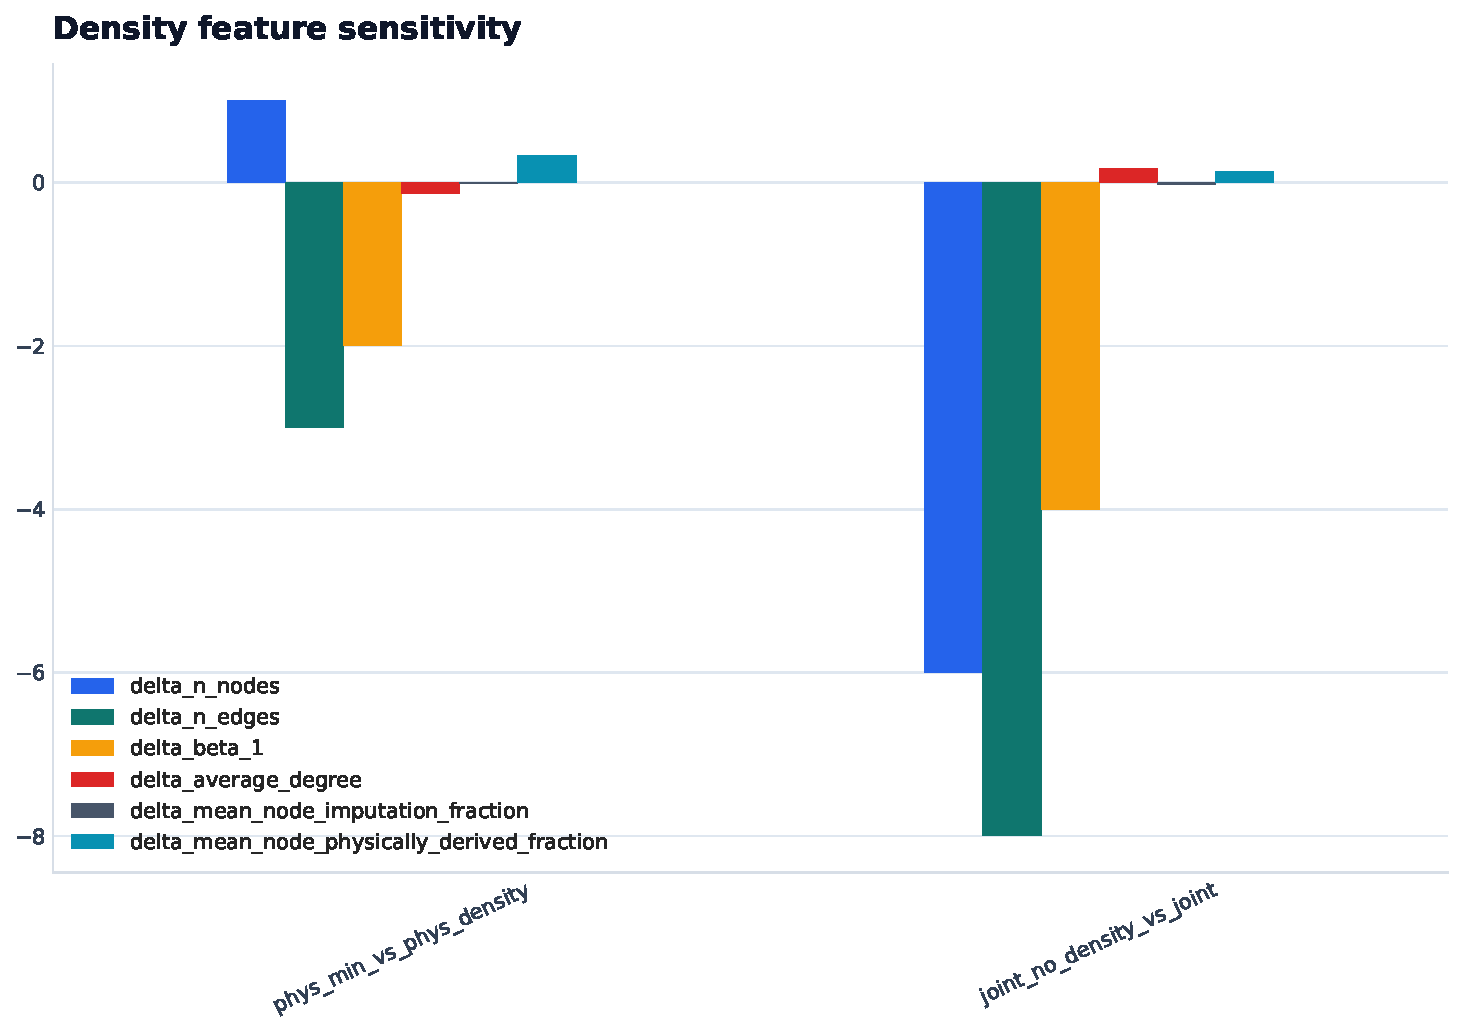
\includegraphics[width=0.9\linewidth]{figures/06_mapper_density_feature_sensitivity.pdf}\caption{Sensibilidad al agregar pl\_dens.}\end{figure}\begin{figure}[H]\centering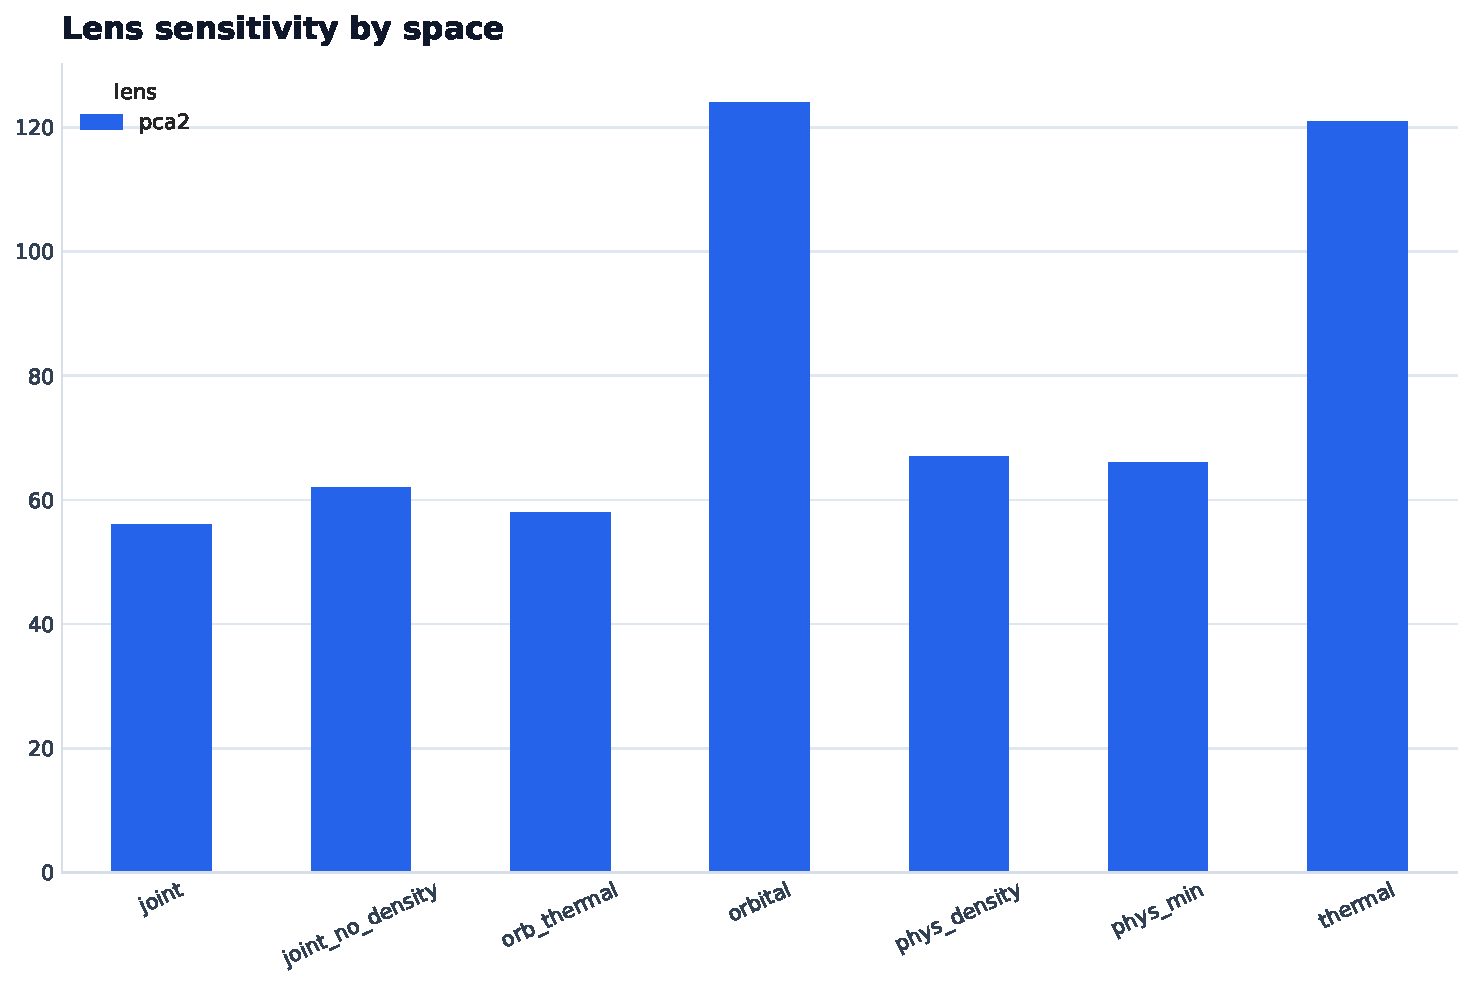
\includegraphics[width=0.9\linewidth]{figures/07_mapper_lens_sensitivity.pdf}\caption{Sensibilidad al lens.}\end{figure}\begin{figure}[H]\centering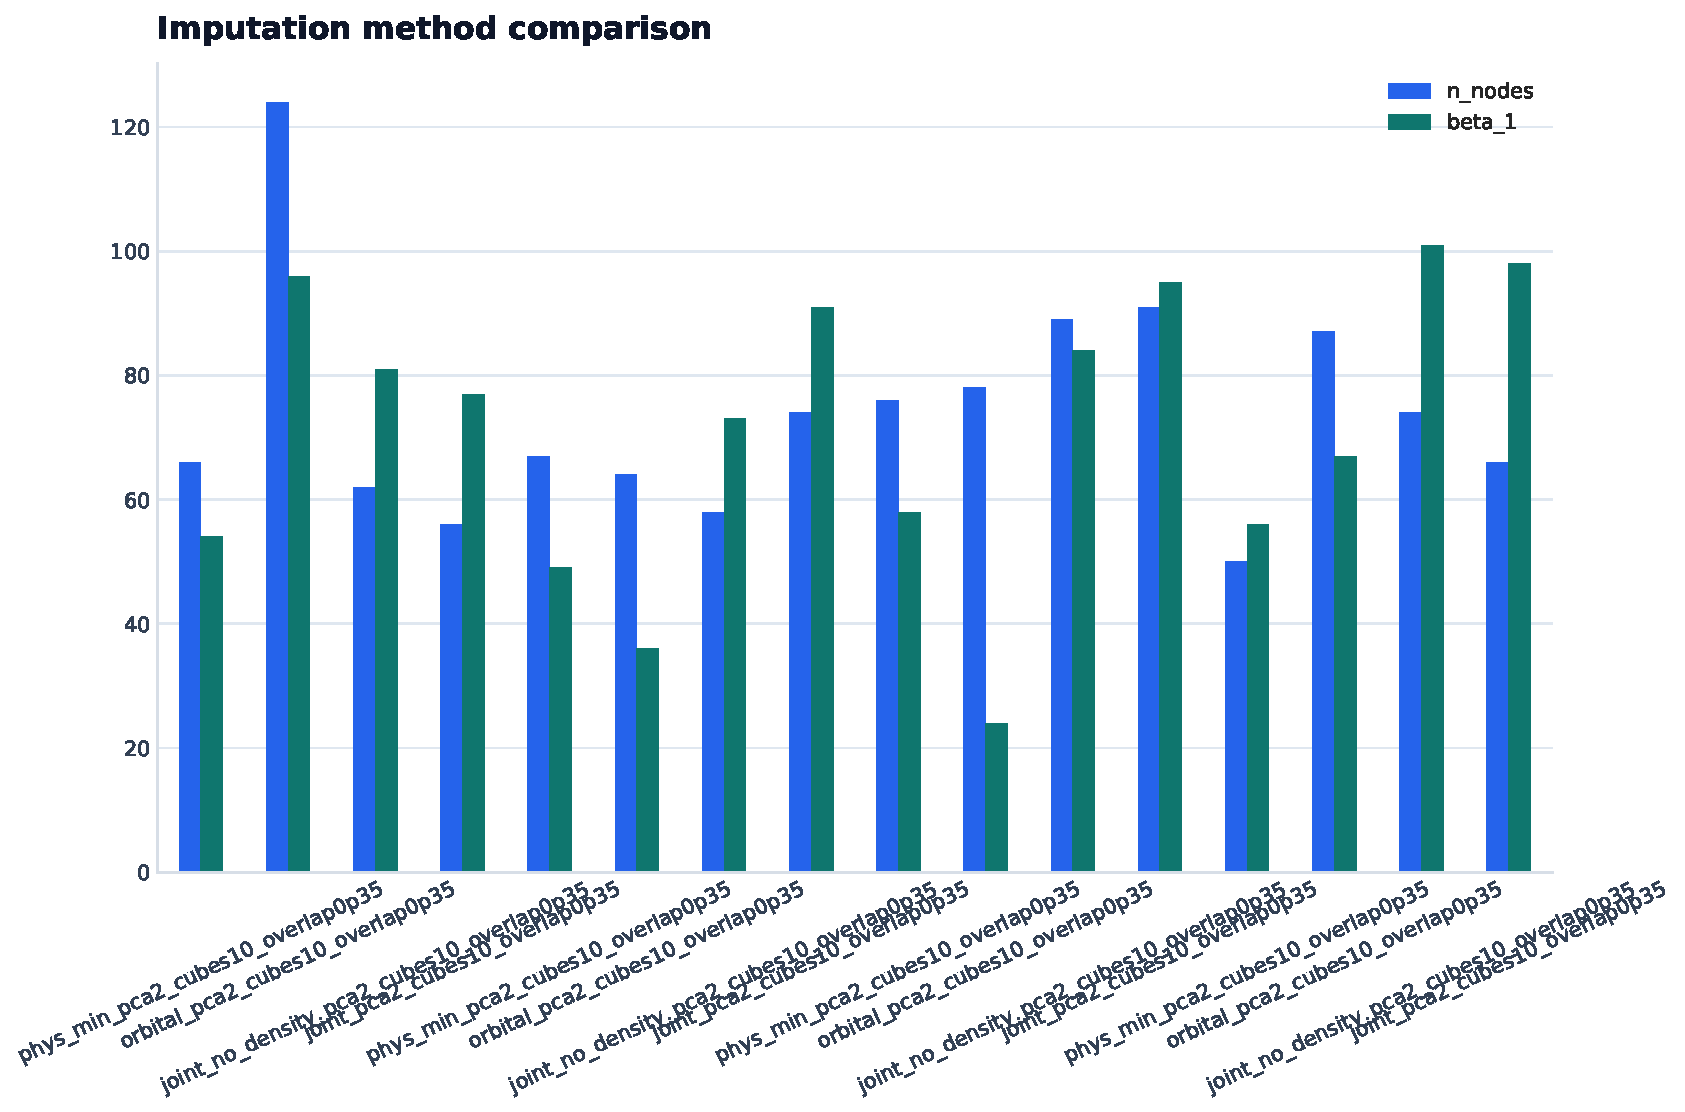
\includegraphics[width=0.9\linewidth]{figures/11_imputation_method_comparison.pdf}\caption{Comparacion entre metodos de imputacion cuando esta disponible.}\end{figure}
